% Options for packages loaded elsewhere
\PassOptionsToPackage{unicode}{hyperref}
\PassOptionsToPackage{hyphens}{url}
%
\documentclass[
  letterpaper,
  DIV=11,
  numbers=noendperiod]{scrartcl}

\usepackage{amsmath,amssymb}
\usepackage{iftex}
\ifPDFTeX
  \usepackage[T1]{fontenc}
  \usepackage[utf8]{inputenc}
  \usepackage{textcomp} % provide euro and other symbols
\else % if luatex or xetex
  \usepackage{unicode-math}
  \defaultfontfeatures{Scale=MatchLowercase}
  \defaultfontfeatures[\rmfamily]{Ligatures=TeX,Scale=1}
\fi
\usepackage{lmodern}
\ifPDFTeX\else  
    % xetex/luatex font selection
\fi
% Use upquote if available, for straight quotes in verbatim environments
\IfFileExists{upquote.sty}{\usepackage{upquote}}{}
\IfFileExists{microtype.sty}{% use microtype if available
  \usepackage[]{microtype}
  \UseMicrotypeSet[protrusion]{basicmath} % disable protrusion for tt fonts
}{}
\makeatletter
\@ifundefined{KOMAClassName}{% if non-KOMA class
  \IfFileExists{parskip.sty}{%
    \usepackage{parskip}
  }{% else
    \setlength{\parindent}{0pt}
    \setlength{\parskip}{6pt plus 2pt minus 1pt}}
}{% if KOMA class
  \KOMAoptions{parskip=half}}
\makeatother
\usepackage{xcolor}
\setlength{\emergencystretch}{3em} % prevent overfull lines
\setcounter{secnumdepth}{-\maxdimen} % remove section numbering
% Make \paragraph and \subparagraph free-standing
\makeatletter
\ifx\paragraph\undefined\else
  \let\oldparagraph\paragraph
  \renewcommand{\paragraph}{
    \@ifstar
      \xxxParagraphStar
      \xxxParagraphNoStar
  }
  \newcommand{\xxxParagraphStar}[1]{\oldparagraph*{#1}\mbox{}}
  \newcommand{\xxxParagraphNoStar}[1]{\oldparagraph{#1}\mbox{}}
\fi
\ifx\subparagraph\undefined\else
  \let\oldsubparagraph\subparagraph
  \renewcommand{\subparagraph}{
    \@ifstar
      \xxxSubParagraphStar
      \xxxSubParagraphNoStar
  }
  \newcommand{\xxxSubParagraphStar}[1]{\oldsubparagraph*{#1}\mbox{}}
  \newcommand{\xxxSubParagraphNoStar}[1]{\oldsubparagraph{#1}\mbox{}}
\fi
\makeatother

\usepackage{color}
\usepackage{fancyvrb}
\newcommand{\VerbBar}{|}
\newcommand{\VERB}{\Verb[commandchars=\\\{\}]}
\DefineVerbatimEnvironment{Highlighting}{Verbatim}{commandchars=\\\{\}}
% Add ',fontsize=\small' for more characters per line
\usepackage{framed}
\definecolor{shadecolor}{RGB}{241,243,245}
\newenvironment{Shaded}{\begin{snugshade}}{\end{snugshade}}
\newcommand{\AlertTok}[1]{\textcolor[rgb]{0.68,0.00,0.00}{#1}}
\newcommand{\AnnotationTok}[1]{\textcolor[rgb]{0.37,0.37,0.37}{#1}}
\newcommand{\AttributeTok}[1]{\textcolor[rgb]{0.40,0.45,0.13}{#1}}
\newcommand{\BaseNTok}[1]{\textcolor[rgb]{0.68,0.00,0.00}{#1}}
\newcommand{\BuiltInTok}[1]{\textcolor[rgb]{0.00,0.23,0.31}{#1}}
\newcommand{\CharTok}[1]{\textcolor[rgb]{0.13,0.47,0.30}{#1}}
\newcommand{\CommentTok}[1]{\textcolor[rgb]{0.37,0.37,0.37}{#1}}
\newcommand{\CommentVarTok}[1]{\textcolor[rgb]{0.37,0.37,0.37}{\textit{#1}}}
\newcommand{\ConstantTok}[1]{\textcolor[rgb]{0.56,0.35,0.01}{#1}}
\newcommand{\ControlFlowTok}[1]{\textcolor[rgb]{0.00,0.23,0.31}{\textbf{#1}}}
\newcommand{\DataTypeTok}[1]{\textcolor[rgb]{0.68,0.00,0.00}{#1}}
\newcommand{\DecValTok}[1]{\textcolor[rgb]{0.68,0.00,0.00}{#1}}
\newcommand{\DocumentationTok}[1]{\textcolor[rgb]{0.37,0.37,0.37}{\textit{#1}}}
\newcommand{\ErrorTok}[1]{\textcolor[rgb]{0.68,0.00,0.00}{#1}}
\newcommand{\ExtensionTok}[1]{\textcolor[rgb]{0.00,0.23,0.31}{#1}}
\newcommand{\FloatTok}[1]{\textcolor[rgb]{0.68,0.00,0.00}{#1}}
\newcommand{\FunctionTok}[1]{\textcolor[rgb]{0.28,0.35,0.67}{#1}}
\newcommand{\ImportTok}[1]{\textcolor[rgb]{0.00,0.46,0.62}{#1}}
\newcommand{\InformationTok}[1]{\textcolor[rgb]{0.37,0.37,0.37}{#1}}
\newcommand{\KeywordTok}[1]{\textcolor[rgb]{0.00,0.23,0.31}{\textbf{#1}}}
\newcommand{\NormalTok}[1]{\textcolor[rgb]{0.00,0.23,0.31}{#1}}
\newcommand{\OperatorTok}[1]{\textcolor[rgb]{0.37,0.37,0.37}{#1}}
\newcommand{\OtherTok}[1]{\textcolor[rgb]{0.00,0.23,0.31}{#1}}
\newcommand{\PreprocessorTok}[1]{\textcolor[rgb]{0.68,0.00,0.00}{#1}}
\newcommand{\RegionMarkerTok}[1]{\textcolor[rgb]{0.00,0.23,0.31}{#1}}
\newcommand{\SpecialCharTok}[1]{\textcolor[rgb]{0.37,0.37,0.37}{#1}}
\newcommand{\SpecialStringTok}[1]{\textcolor[rgb]{0.13,0.47,0.30}{#1}}
\newcommand{\StringTok}[1]{\textcolor[rgb]{0.13,0.47,0.30}{#1}}
\newcommand{\VariableTok}[1]{\textcolor[rgb]{0.07,0.07,0.07}{#1}}
\newcommand{\VerbatimStringTok}[1]{\textcolor[rgb]{0.13,0.47,0.30}{#1}}
\newcommand{\WarningTok}[1]{\textcolor[rgb]{0.37,0.37,0.37}{\textit{#1}}}

\providecommand{\tightlist}{%
  \setlength{\itemsep}{0pt}\setlength{\parskip}{0pt}}\usepackage{longtable,booktabs,array}
\usepackage{calc} % for calculating minipage widths
% Correct order of tables after \paragraph or \subparagraph
\usepackage{etoolbox}
\makeatletter
\patchcmd\longtable{\par}{\if@noskipsec\mbox{}\fi\par}{}{}
\makeatother
% Allow footnotes in longtable head/foot
\IfFileExists{footnotehyper.sty}{\usepackage{footnotehyper}}{\usepackage{footnote}}
\makesavenoteenv{longtable}
\usepackage{graphicx}
\makeatletter
\def\maxwidth{\ifdim\Gin@nat@width>\linewidth\linewidth\else\Gin@nat@width\fi}
\def\maxheight{\ifdim\Gin@nat@height>\textheight\textheight\else\Gin@nat@height\fi}
\makeatother
% Scale images if necessary, so that they will not overflow the page
% margins by default, and it is still possible to overwrite the defaults
% using explicit options in \includegraphics[width, height, ...]{}
\setkeys{Gin}{width=\maxwidth,height=\maxheight,keepaspectratio}
% Set default figure placement to htbp
\makeatletter
\def\fps@figure{htbp}
\makeatother

\KOMAoption{captions}{tableheading}
\makeatletter
\@ifpackageloaded{caption}{}{\usepackage{caption}}
\AtBeginDocument{%
\ifdefined\contentsname
  \renewcommand*\contentsname{Tabla de contenidos}
\else
  \newcommand\contentsname{Tabla de contenidos}
\fi
\ifdefined\listfigurename
  \renewcommand*\listfigurename{Listado de Figuras}
\else
  \newcommand\listfigurename{Listado de Figuras}
\fi
\ifdefined\listtablename
  \renewcommand*\listtablename{Listado de Tablas}
\else
  \newcommand\listtablename{Listado de Tablas}
\fi
\ifdefined\figurename
  \renewcommand*\figurename{Figura}
\else
  \newcommand\figurename{Figura}
\fi
\ifdefined\tablename
  \renewcommand*\tablename{Tabla}
\else
  \newcommand\tablename{Tabla}
\fi
}
\@ifpackageloaded{float}{}{\usepackage{float}}
\floatstyle{ruled}
\@ifundefined{c@chapter}{\newfloat{codelisting}{h}{lop}}{\newfloat{codelisting}{h}{lop}[chapter]}
\floatname{codelisting}{Listado}
\newcommand*\listoflistings{\listof{codelisting}{Listado de Listados}}
\makeatother
\makeatletter
\makeatother
\makeatletter
\@ifpackageloaded{caption}{}{\usepackage{caption}}
\@ifpackageloaded{subcaption}{}{\usepackage{subcaption}}
\makeatother

\ifLuaTeX
\usepackage[bidi=basic]{babel}
\else
\usepackage[bidi=default]{babel}
\fi
\babelprovide[main,import]{spanish}
% get rid of language-specific shorthands (see #6817):
\let\LanguageShortHands\languageshorthands
\def\languageshorthands#1{}
\ifLuaTeX
  \usepackage{selnolig}  % disable illegal ligatures
\fi
\usepackage{bookmark}

\IfFileExists{xurl.sty}{\usepackage{xurl}}{} % add URL line breaks if available
\urlstyle{same} % disable monospaced font for URLs
\hypersetup{
  pdftitle={Trabajo Practico 1: El modelo de visualización de Ben Fry},
  pdfauthor={Andrea Gomez Vargas},
  pdflang={es},
  hidelinks,
  pdfcreator={LaTeX via pandoc}}


\title{Trabajo Practico 1: El modelo de visualización de Ben Fry}
\usepackage{etoolbox}
\makeatletter
\providecommand{\subtitle}[1]{% add subtitle to \maketitle
  \apptocmd{\@title}{\par {\large #1 \par}}{}{}
}
\makeatother
\subtitle{Maestría en Generación y Análisis de Información Estadística -
UNTREF}
\author{Andrea Gomez Vargas}
\date{22/10/2026}

\begin{document}
\maketitle

\renewcommand*\contentsname{Tabla de contenidos}
{
\setcounter{tocdepth}{3}
\tableofcontents
}

\newpage

\section{Nuevos argentinos: un análisis de las nacionalizaciones en
Argentina, años
2013--2024}\label{nuevos-argentinos-un-anuxe1lisis-de-las-nacionalizaciones-en-argentina-auxf1os-20132024}

\subsection{Introducción: la nacionalización en
Argentina}\label{introducciuxf3n-la-nacionalizaciuxf3n-en-argentina}

La nacionalización es un proceso voluntario por el cual una persona
nacida en el extranjero adquiere la nacionalidad argentina y, con ella,
la pertenencia jurídico-política a la nación. Está regida por la Ley N°
346 de Ciudadanía y Naturalización (1869) y su decreto reglamentario N°
3213/1984 (actualizado por última vez en 2004). Bajo este marco existen
dos vías de acceso: la carta de ciudadanía, habitualmente conocida como
``naturalización'', y la opción.

\subsubsection{Nacionalización por carta de
ciudadanía}\label{nacionalizaciuxf3n-por-carta-de-ciudadanuxeda}

Es la vía por la cual la población extranjera residente en Argentina
puede adquirir la nacionalidad. Se trata de un procedimiento judicial
que la persona inicia voluntariamente y que culmina con el otorgamiento
de la carta de ciudadanía. Una vez obtenida, la persona debe tramitar
ante el Registro Nacional de las Personas (RENAPER) su primer Documento
Nacional de Identidad (DNI) como argentina.

\subsubsection{Nacionalización por
opción}\label{nacionalizaciuxf3n-por-opciuxf3n}

Corresponde a personas nacidas en el extranjero que son hijas de padre o
madre argentino nativo. Es un trámite administrativo que se realiza en
los consulados argentinos, si la persona reside fuera del país, o en las
oficinas del RENAPER y los registros civiles, si se encuentra en
Argentina.

La distinción entre ambas vías es relevante para el análisis: la carta
de ciudadanía refleja trayectorias de inmigración y residencia en el
país, mientras que la opción expresa vínculos de filiación con la
población argentina, incluida la emigrada.

\subsection{Pregunta de interés}\label{pregunta-de-interuxe9s}

\begin{quote}
¿Desde qué países de origen y por qué vía de acceso (carta de ciudadanía
u opción) se nacionalizaron las personas en Argentina entre 2013 y 2024,
y cómo evolucionaron los principales orígenes en ese período?
\end{quote}

La pregunta busca identificar qué países concentran las
nacionalizaciones, si esa composición difiere según la vía de acceso y
cómo cambiaron a lo largo del tiempo los cinco principales países de
origen.

\subsection{Fuente de datos}\label{fuente-de-datos}

Se utiliza la base \emph{Población nacionalizada en Argentina},
elaborada por la Dirección Nacional de Población a partir de los
registros administrativos del RENAPER y publicada en el portal de datos
abiertos del Estado nacional:

\begin{itemize}
\tightlist
\item
  Dataset:
  \url{https://datos.gob.ar/dataset/poblacion-nacionalizada-en-argentina}
\item
  Página de referencia:
  \url{https://www.argentina.gob.ar/interior/renaper/estadistica-de-poblacion}
\end{itemize}

La base contiene la cantidad de personas que obtuvieron la nacionalidad
argentina y realizaron su primer DNI, según tipo de nacionalización,
país de nacimiento y año de trámite, entre el 1 de enero de 2013 y el 20
de agosto de 2025.

El registro se apoya en el proceso de digitalización de la
identificación de personas iniciado con el Decreto N° 1501/2009, que
estableció la emisión digital del DNI para ciudadanos nacionales y
extranjeros (Resoluciones RENAPER N° 1800/2009 y N° 585/2012).

\subsubsection{Unidad de análisis y
periodo}\label{unidad-de-anuxe1lisis-y-periodo}

Personas nacionalizadas que realizaron, entre el 1 de enero de 2013 y el
31 de diciembre de 2024, el trámite de su primer DNI como argentinas
ante el RENAPER.

\subsubsection{Alcances y limitaciones}\label{alcances-y-limitaciones}

\begin{itemize}
\tightlist
\item
  \textbf{Cobertura del registro.} Solo se contabilizan personas que
  tramitaron su primer DNI digital como argentinas. Quedan excluidas
  quienes tienen documentos confeccionados manualmente (Libreta Cívica,
  Libreta de Enrolamiento, DNI tapa verde o bordó) y quienes tramitaron
  el DNI digital fuera del período.
\item
  \textbf{Fecha de referencia.} El año corresponde al trámite del primer
  DNI, no a la fecha de otorgamiento de la nacionalidad. Puede haber un
  desfasaje entre ambos momentos, especialmente en la vía judicial.
\item
  \textbf{Nacionalizaciones sin DNI.} Las personas que obtuvieron la
  nacionalidad pero no tramitaron su primer DNI argentino no aparecen en
  la base.
\item
  \textbf{Período analizado.} Aunque la base llega hasta el 20 de agosto
  de 2025, se excluye ese año por contener datos parciales, para
  trabajar solo con años completos y comparables.
\end{itemize}

\subsection{Modelo de visualización de Ben
Fry}\label{modelo-de-visualizaciuxf3n-de-ben-fry}

Ben Fry (2008) propone siete etapas para desarrollar una visualización
de datos: obtener, estructurar, filtrar, explorar, representar, refinar
e interactuar. Este trabajo desarrolla las seis primeras; la última
(\emph{Interact}) queda fuera porque el producto final es una
visualización estática.

\subsubsection{\texorpdfstring{1. Obtener
(\emph{Acquire})}{1. Obtener (Acquire)}}\label{obtener-acquire}

El dataset se obtiene desde el portal de datos abierto a través de la
URL del recurso:
\url{https://datosabiertos.renaper.gob.ar/Cantidad_de_tramites_de_DNI_argentino_por_nacionalidad_pais_anio.csv}

\begin{Shaded}
\begin{Highlighting}[]
\CommentTok{\# prepararo paquetes de trabajo}

\FunctionTok{library}\NormalTok{(tidyverse)}
\FunctionTok{library}\NormalTok{(janitor)}
\FunctionTok{library}\NormalTok{(scales)}
\FunctionTok{library}\NormalTok{(knitr)}
\FunctionTok{library}\NormalTok{(tidytext)}
\end{Highlighting}
\end{Shaded}

\begin{Shaded}
\begin{Highlighting}[]
\NormalTok{renaper }\OtherTok{\textless{}{-}} \FunctionTok{paste0}\NormalTok{(}
  \StringTok{"https://datosabiertos.renaper.gob.ar/"}\NormalTok{,}
  \StringTok{"Cantidad\_de\_tramites\_de\_DNI\_argentino\_"}\NormalTok{,}
  \StringTok{"por\_nacionalidad\_pais\_anio.csv"}
\NormalTok{)}

\NormalTok{pob\_nacionalizada }\OtherTok{\textless{}{-}} \FunctionTok{read\_csv}\NormalTok{(renaper, }\AttributeTok{show\_col\_types =} \ConstantTok{FALSE}\NormalTok{)}

\DocumentationTok{\#\# Lectura de composición del  dataset}
\FunctionTok{glimpse}\NormalTok{(pob\_nacionalizada)}
\end{Highlighting}
\end{Shaded}

\begin{verbatim}
Rows: 1,974
Columns: 4
$ pais_nac          <chr> "ALBANIA", "ALBANIA", "ALBANIA", "ALBANIA", "ALBANIA~
$ Tipo_nacionalidad <chr> "CARTA", "CARTA", "CARTA", "CARTA", "CARTA", "CARTA"~
$ anio              <dbl> 2013, 2014, 2017, 2019, 2020, 2024, 2021, 2023, 2013~
$ cantidad          <dbl> 1, 1, 2, 1, 2, 2, 1, 4, 5, 8, 5, 5, 7, 6, 4, 2, 3, 2~
\end{verbatim}

La base cuenta con 1.974 observaciones y 4 variables: país de nacimiento
(\texttt{pais\_nac}), vía de acceso a la nacionalidad
(\texttt{Tipo\_nacionalidad}) con las categorías CARTA y OPCION, año de
trámite del primer DNI (\texttt{anio}) y cantidad de personas
nacionalizadas (\texttt{cantidad}). Cada fila corresponde a una
combinación de país, vía de acceso y año; las combinaciones sin casos no
figuran en la base.

\subsubsection{\texorpdfstring{2. Estructurar
(\emph{Parse})}{2. Estructurar (Parse)}}\label{estructurar-parse}

Se estandarizan los nombres de las variables, se ajusta el año a número
entero y se recodifican las categorías para que sean legibles en el
gráfico.

\begin{Shaded}
\begin{Highlighting}[]
\NormalTok{nac }\OtherTok{\textless{}{-}}\NormalTok{ pob\_nacionalizada }\SpecialCharTok{|\textgreater{}}
  \FunctionTok{clean\_names}\NormalTok{() }\SpecialCharTok{|\textgreater{}} 
  \FunctionTok{mutate}\NormalTok{(}
    \AttributeTok{anio =} \FunctionTok{as.integer}\NormalTok{(anio),}
    \AttributeTok{tipo =} \FunctionTok{recode}\NormalTok{(tipo\_nacionalidad,}
                  \StringTok{"CARTA"}  \OtherTok{=} \StringTok{"Carta de ciudadanía"}\NormalTok{,}
                  \StringTok{"OPCION"} \OtherTok{=} \StringTok{"Opción"}\NormalTok{),}
    \AttributeTok{pais =} \FunctionTok{str\_to\_title}\NormalTok{(pais\_nac),}
    \AttributeTok{pais =} \FunctionTok{case\_when}\NormalTok{(}
\NormalTok{                    pais }\SpecialCharTok{==} \StringTok{"Peru"} \SpecialCharTok{\textasciitilde{}} \StringTok{"Perú"}\NormalTok{,}
\NormalTok{                    pais }\SpecialCharTok{==} \StringTok{"Mexico"} \SpecialCharTok{\textasciitilde{}} \StringTok{"México"}\NormalTok{,}
\NormalTok{                    pais }\SpecialCharTok{==} \StringTok{"Republica Dominicana"} \SpecialCharTok{\textasciitilde{}} \StringTok{"República Dominicana"}\NormalTok{,}
                    \AttributeTok{.default =}\NormalTok{ pais}
\NormalTok{                  )}
\NormalTok{  )}
\end{Highlighting}
\end{Shaded}

\subsubsection{\texorpdfstring{3. Filtrar
(\emph{Filter})}{3. Filtrar (Filter)}}\label{filtrar-filter}

Se restringe el período a los años completos (2013--2024), excluyendo
2025 por contener datos solo hasta el 20 de agosto.

\begin{Shaded}
\begin{Highlighting}[]
\NormalTok{nac\_periodo }\OtherTok{\textless{}{-}}\NormalTok{ nac }\SpecialCharTok{|\textgreater{}}
  \FunctionTok{filter}\NormalTok{(}\FunctionTok{between}\NormalTok{(anio, }\DecValTok{2013}\NormalTok{, }\DecValTok{2024}\NormalTok{))}
\end{Highlighting}
\end{Shaded}

Para poder comparar los perfiles de origen según la vía de acceso, la
selección se realiza por separado para carta de ciudadanía y para
opción. Para cada vía se identifican los diez países con mayor cantidad
de personas nacionalizadas en el período.

\begin{Shaded}
\begin{Highlighting}[]
\NormalTok{datos\_a }\OtherTok{\textless{}{-}}\NormalTok{ nac\_periodo }\SpecialCharTok{|\textgreater{}}
  \FunctionTok{group\_by}\NormalTok{(tipo, pais) }\SpecialCharTok{|\textgreater{}}
  \FunctionTok{summarise}\NormalTok{(}
    \AttributeTok{total =} \FunctionTok{sum}\NormalTok{(cantidad),}
    \AttributeTok{.groups =} \StringTok{"drop\_last"}
\NormalTok{  ) }\SpecialCharTok{|\textgreater{}}
  \FunctionTok{slice\_max}\NormalTok{(total, }\AttributeTok{n =} \DecValTok{10}\NormalTok{, }\AttributeTok{with\_ties =} \ConstantTok{FALSE}\NormalTok{) }\SpecialCharTok{|\textgreater{}}
  \FunctionTok{ungroup}\NormalTok{()}

\FunctionTok{kable}\NormalTok{(datos\_a)}
\end{Highlighting}
\end{Shaded}

\begin{longtable}[]{@{}llr@{}}
\toprule\noalign{}
tipo & pais & total \\
\midrule\noalign{}
\endhead
\bottomrule\noalign{}
\endlastfoot
Carta de ciudadanía & Venezuela & 12112 \\
Carta de ciudadanía & Perú & 8249 \\
Carta de ciudadanía & Bolivia & 7774 \\
Carta de ciudadanía & República Dominicana & 5576 \\
Carta de ciudadanía & Paraguay & 4638 \\
Carta de ciudadanía & Chile & 4410 \\
Carta de ciudadanía & Colombia & 2232 \\
Carta de ciudadanía & Cuba & 1991 \\
Carta de ciudadanía & Senegal & 1496 \\
Carta de ciudadanía & Rusia & 1338 \\
Opción & España & 8290 \\
Opción & Estados Unidos & 5679 \\
Opción & Chile & 4065 \\
Opción & Brasil & 3441 \\
Opción & Bolivia & 3177 \\
Opción & Venezuela & 3125 \\
Opción & Paraguay & 3054 \\
Opción & México & 1847 \\
Opción & Italia & 1811 \\
Opción & Israel & 1728 \\
\end{longtable}

Para la serie temporal se toman los cinco primeros países de cada vía, y
se arma su evolución anual. Los años sin registros se completan con cero
para que las líneas no omitan esos años.

\begin{Shaded}
\begin{Highlighting}[]
\NormalTok{top5\_tipo }\OtherTok{\textless{}{-}}\NormalTok{ datos\_a }\SpecialCharTok{|\textgreater{}}
  \FunctionTok{group\_by}\NormalTok{(tipo) }\SpecialCharTok{|\textgreater{}}
  \FunctionTok{slice\_max}\NormalTok{(total, }\AttributeTok{n =} \DecValTok{5}\NormalTok{, }\AttributeTok{with\_ties =} \ConstantTok{FALSE}\NormalTok{) }\SpecialCharTok{|\textgreater{}}
  \FunctionTok{ungroup}\NormalTok{()}

\NormalTok{datos\_b }\OtherTok{\textless{}{-}}\NormalTok{ nac\_periodo }\SpecialCharTok{|\textgreater{}}
  \FunctionTok{semi\_join}\NormalTok{(top5\_tipo, }\AttributeTok{by =} \FunctionTok{c}\NormalTok{(}\StringTok{"tipo"}\NormalTok{, }\StringTok{"pais"}\NormalTok{)) }\SpecialCharTok{|\textgreater{}}
  \FunctionTok{group\_by}\NormalTok{(tipo, pais, anio) }\SpecialCharTok{|\textgreater{}}
  \FunctionTok{summarise}\NormalTok{(}
    \AttributeTok{cantidad =} \FunctionTok{sum}\NormalTok{(cantidad),}
    \AttributeTok{.groups =} \StringTok{"drop"}
\NormalTok{  ) }\SpecialCharTok{|\textgreater{}}
  \FunctionTok{complete}\NormalTok{(}
    \FunctionTok{nesting}\NormalTok{(tipo, pais),}
    \AttributeTok{anio =} \DecValTok{2013}\SpecialCharTok{:}\DecValTok{2024}\NormalTok{,}
    \AttributeTok{fill =} \FunctionTok{list}\NormalTok{(}\AttributeTok{cantidad =} \DecValTok{0}\NormalTok{)}
\NormalTok{  )}
\end{Highlighting}
\end{Shaded}

Como resultado de esta etapa se obtienen dos conjuntos de datos: el
primero reúne a los diez principales países de cada vía de acceso con su
total del período; el segundo contiene la serie anual de los cinco
principales países de cada vía.

\subsubsection{\texorpdfstring{4. Explorar
(\emph{Mine})}{4. Explorar (Mine)}}\label{explorar-mine}

En esta etapa se calculan medidas para identificar patrones antes de
graficar: el volumen de cada vía de acceso, su evolución anual, el grado
de concentración en pocos países, la coincidencia entre los rankings de
ambas vías y la evolución de los principales países.

\paragraph{¿Cuánto pesa cada vía en el
total?}\label{cuuxe1nto-pesa-cada-vuxeda-en-el-total}

\begin{Shaded}
\begin{Highlighting}[]
\NormalTok{totales\_tipo }\OtherTok{\textless{}{-}}\NormalTok{ nac\_periodo }\SpecialCharTok{|\textgreater{}}
  \FunctionTok{group\_by}\NormalTok{(tipo) }\SpecialCharTok{|\textgreater{}}
  \FunctionTok{summarise}\NormalTok{(}
    \AttributeTok{total\_tipo =} \FunctionTok{sum}\NormalTok{(cantidad),}
    \AttributeTok{.groups =} \StringTok{"drop"}
\NormalTok{  )}

\NormalTok{total }\OtherTok{\textless{}{-}}\NormalTok{ totales\_tipo }\SpecialCharTok{|\textgreater{}}
  \FunctionTok{mutate}\NormalTok{(}\AttributeTok{pct =} \FunctionTok{round}\NormalTok{(total\_tipo }\SpecialCharTok{/} \FunctionTok{sum}\NormalTok{(total\_tipo) }\SpecialCharTok{*} \DecValTok{100}\NormalTok{, }\DecValTok{1}\NormalTok{))}

\FunctionTok{kable}\NormalTok{(total)}
\end{Highlighting}
\end{Shaded}

\begin{longtable}[]{@{}lrr@{}}
\toprule\noalign{}
tipo & total\_tipo & pct \\
\midrule\noalign{}
\endhead
\bottomrule\noalign{}
\endlastfoot
Carta de ciudadanía & 59019 & 54.2 \\
Opción & 49899 & 45.8 \\
\end{longtable}

Las dos vías tienen volúmenes comparables: la carta de ciudadanía reúne
59.019 personas (54,2\%) y la opción 49.899 (45,8\%).

\paragraph{¿Cómo evolucionó cada vía año a
año?}\label{cuxf3mo-evolucionuxf3-cada-vuxeda-auxf1o-a-auxf1o}

\begin{Shaded}
\begin{Highlighting}[]
\NormalTok{nac\_periodo }\SpecialCharTok{|\textgreater{}}
  \FunctionTok{group\_by}\NormalTok{(anio, tipo) }\SpecialCharTok{|\textgreater{}}
  \FunctionTok{summarise}\NormalTok{(}
    \AttributeTok{total =} \FunctionTok{sum}\NormalTok{(cantidad),}
    \AttributeTok{.groups =} \StringTok{"drop"}
\NormalTok{  ) }\SpecialCharTok{|\textgreater{}}
  \FunctionTok{pivot\_wider}\NormalTok{(}\AttributeTok{names\_from =}\NormalTok{ tipo, }\AttributeTok{values\_from =}\NormalTok{ total) }\SpecialCharTok{|\textgreater{}} 
  \FunctionTok{kable}\NormalTok{()}
\end{Highlighting}
\end{Shaded}

\begin{longtable}[]{@{}rrr@{}}
\toprule\noalign{}
anio & Carta de ciudadanía & Opción \\
\midrule\noalign{}
\endhead
\bottomrule\noalign{}
\endlastfoot
2013 & 4655 & 4416 \\
2014 & 4484 & 3970 \\
2015 & 4818 & 3925 \\
2016 & 4626 & 4195 \\
2017 & 4427 & 4461 \\
2018 & 4471 & 4588 \\
2019 & 4437 & 4130 \\
2020 & 1622 & 1519 \\
2021 & 3569 & 2878 \\
2022 & 5311 & 4373 \\
2023 & 7351 & 5508 \\
2024 & 9248 & 5936 \\
\end{longtable}

Entre 2013 y 2019 ambas vías se mantienen estables, en torno a
4.000--4.800 personas por año. En 2020 caen a alrededor de un tercio, en
coincidencia con la pandemia. A partir de 2022 la recuperación es
marcada: en 2024 la carta de ciudadanía prácticamente duplica su nivel
de 2013 (9.248 frente a 4.655), mientras que la opción crece un 34\%.

\paragraph{¿Qué tan concentradas están las nacionalizaciones en cada
vía?}\label{quuxe9-tan-concentradas-estuxe1n-las-nacionalizaciones-en-cada-vuxeda}

\begin{Shaded}
\begin{Highlighting}[]
\NormalTok{datos\_a }\SpecialCharTok{|\textgreater{}}
  \FunctionTok{left\_join}\NormalTok{(totales\_tipo, }\AttributeTok{by =} \StringTok{"tipo"}\NormalTok{) }\SpecialCharTok{|\textgreater{}}
  \FunctionTok{group\_by}\NormalTok{(tipo) }\SpecialCharTok{|\textgreater{}}
  \FunctionTok{mutate}\NormalTok{(}
    \AttributeTok{pct      =} \FunctionTok{round}\NormalTok{(total }\SpecialCharTok{/}\NormalTok{ total\_tipo }\SpecialCharTok{*} \DecValTok{100}\NormalTok{, }\DecValTok{1}\NormalTok{),}
    \AttributeTok{pct\_acum =} \FunctionTok{cumsum}\NormalTok{(pct)}
\NormalTok{  ) }\SpecialCharTok{|\textgreater{}}
  \FunctionTok{ungroup}\NormalTok{() }\SpecialCharTok{|\textgreater{}}
  \FunctionTok{select}\NormalTok{(}\SpecialCharTok{{-}}\NormalTok{total\_tipo) }\SpecialCharTok{|\textgreater{}} 
  \FunctionTok{kable}\NormalTok{()}
\end{Highlighting}
\end{Shaded}

\begin{longtable}[]{@{}llrrr@{}}
\toprule\noalign{}
tipo & pais & total & pct & pct\_acum \\
\midrule\noalign{}
\endhead
\bottomrule\noalign{}
\endlastfoot
Carta de ciudadanía & Venezuela & 12112 & 20.5 & 20.5 \\
Carta de ciudadanía & Perú & 8249 & 14.0 & 34.5 \\
Carta de ciudadanía & Bolivia & 7774 & 13.2 & 47.7 \\
Carta de ciudadanía & República Dominicana & 5576 & 9.4 & 57.1 \\
Carta de ciudadanía & Paraguay & 4638 & 7.9 & 65.0 \\
Carta de ciudadanía & Chile & 4410 & 7.5 & 72.5 \\
Carta de ciudadanía & Colombia & 2232 & 3.8 & 76.3 \\
Carta de ciudadanía & Cuba & 1991 & 3.4 & 79.7 \\
Carta de ciudadanía & Senegal & 1496 & 2.5 & 82.2 \\
Carta de ciudadanía & Rusia & 1338 & 2.3 & 84.5 \\
Opción & España & 8290 & 16.6 & 16.6 \\
Opción & Estados Unidos & 5679 & 11.4 & 28.0 \\
Opción & Chile & 4065 & 8.1 & 36.1 \\
Opción & Brasil & 3441 & 6.9 & 43.0 \\
Opción & Bolivia & 3177 & 6.4 & 49.4 \\
Opción & Venezuela & 3125 & 6.3 & 55.7 \\
Opción & Paraguay & 3054 & 6.1 & 61.8 \\
Opción & México & 1847 & 3.7 & 65.5 \\
Opción & Italia & 1811 & 3.6 & 69.1 \\
Opción & Israel & 1728 & 3.5 & 72.6 \\
\end{longtable}

La carta de ciudadanía está más concentrada: sus diez principales países
reúnen el 84,5\% del total de la vía, y los tres primeros casi la mitad.
En opción, los diez principales reúnen el 72,6\%.El porcentaje se
calcula sobre el total de cada vía, con todos los países. La última fila
de cada vía indica cuánto concentran sus diez principales países

\paragraph{¿Qué países aparecen en las dos
vías?}\label{quuxe9-pauxedses-aparecen-en-las-dos-vuxedas}

\begin{Shaded}
\begin{Highlighting}[]
\NormalTok{datos\_a }\SpecialCharTok{|\textgreater{}}
  \FunctionTok{count}\NormalTok{(pais) }\SpecialCharTok{|\textgreater{}}
  \FunctionTok{filter}\NormalTok{(n }\SpecialCharTok{==} \DecValTok{2}\NormalTok{) }\SpecialCharTok{|\textgreater{}} 
  \FunctionTok{kable}\NormalTok{()}
\end{Highlighting}
\end{Shaded}

\begin{longtable}[]{@{}lr@{}}
\toprule\noalign{}
pais & n \\
\midrule\noalign{}
\endhead
\bottomrule\noalign{}
\endlastfoot
Bolivia & 2 \\
Chile & 2 \\
Paraguay & 2 \\
Venezuela & 2 \\
\end{longtable}

Solo cuatro países figuran entre los diez principales de ambas vías:
Bolivia, Chile, Paraguay y Venezuela, todos sudamericanos. El resto de
los rankings es distinto: en carta predominan países latinoamericanos y
del Caribe, y en opción aparecen España, Estados Unidos, México, Italia
e Israel.

\paragraph{¿Cómo evolucionaron los cinco principales de cada
vía?}\label{cuxf3mo-evolucionaron-los-cinco-principales-de-cada-vuxeda}

\begin{itemize}
\tightlist
\item
  Variaciones del primer al ultimo año de análisis
\end{itemize}

\begin{Shaded}
\begin{Highlighting}[]
\NormalTok{datos\_b }\SpecialCharTok{|\textgreater{}}
  \FunctionTok{filter}\NormalTok{(anio }\SpecialCharTok{\%in\%} \FunctionTok{c}\NormalTok{(}\DecValTok{2013}\NormalTok{, }\DecValTok{2024}\NormalTok{)) }\SpecialCharTok{|\textgreater{}}
  \FunctionTok{pivot\_wider}\NormalTok{(}
    \AttributeTok{names\_from =}\NormalTok{ anio,}
    \AttributeTok{values\_from =}\NormalTok{ cantidad,}
    \AttributeTok{names\_prefix =} \StringTok{"a"}
\NormalTok{  ) }\SpecialCharTok{|\textgreater{}}
  \FunctionTok{mutate}\NormalTok{(}\AttributeTok{var\_pct =} \FunctionTok{round}\NormalTok{((a2024 }\SpecialCharTok{{-}}\NormalTok{ a2013) }\SpecialCharTok{/}\NormalTok{ a2013 }\SpecialCharTok{*} \DecValTok{100}\NormalTok{, }\DecValTok{1}\NormalTok{)) }\SpecialCharTok{|\textgreater{}} 
  \FunctionTok{kable}\NormalTok{()}
\end{Highlighting}
\end{Shaded}

\begin{longtable}[]{@{}llrrr@{}}
\toprule\noalign{}
tipo & pais & a2013 & a2024 & var\_pct \\
\midrule\noalign{}
\endhead
\bottomrule\noalign{}
\endlastfoot
Carta de ciudadanía & Bolivia & 740 & 737 & -0.4 \\
Carta de ciudadanía & Paraguay & 493 & 251 & -49.1 \\
Carta de ciudadanía & Perú & 920 & 678 & -26.3 \\
Carta de ciudadanía & República Dominicana & 361 & 398 & 10.2 \\
Carta de ciudadanía & Venezuela & 19 & 4411 & 23115.8 \\
Opción & Bolivia & 242 & 457 & 88.8 \\
Opción & Brasil & 237 & 289 & 21.9 \\
Opción & Chile & 272 & 595 & 118.8 \\
Opción & España & 1319 & 1037 & -21.4 \\
Opción & Estados Unidos & 353 & 809 & 129.2 \\
\end{longtable}

\begin{itemize}
\tightlist
\item
  Año de mayor impacto por país
\end{itemize}

\begin{Shaded}
\begin{Highlighting}[]
\CommentTok{\# Año de máximo de cada país}
\NormalTok{datos\_b }\SpecialCharTok{|\textgreater{}}
  \FunctionTok{group\_by}\NormalTok{(tipo, pais) }\SpecialCharTok{|\textgreater{}}
  \FunctionTok{slice\_max}\NormalTok{(cantidad, }\AttributeTok{n =} \DecValTok{1}\NormalTok{, }\AttributeTok{with\_ties =} \ConstantTok{FALSE}\NormalTok{) }\SpecialCharTok{|\textgreater{}}
  \FunctionTok{ungroup}\NormalTok{() }\SpecialCharTok{|\textgreater{}} 
  \FunctionTok{kable}\NormalTok{()}
\end{Highlighting}
\end{Shaded}

\begin{longtable}[]{@{}llrr@{}}
\toprule\noalign{}
tipo & pais & anio & cantidad \\
\midrule\noalign{}
\endhead
\bottomrule\noalign{}
\endlastfoot
Carta de ciudadanía & Bolivia & 2016 & 783 \\
Carta de ciudadanía & Paraguay & 2016 & 533 \\
Carta de ciudadanía & Perú & 2013 & 920 \\
Carta de ciudadanía & República Dominicana & 2015 & 816 \\
Carta de ciudadanía & Venezuela & 2024 & 4411 \\
Opción & Bolivia & 2024 & 457 \\
Opción & Brasil & 2017 & 382 \\
Opción & Chile & 2023 & 612 \\
Opción & España & 2013 & 1319 \\
Opción & Estados Unidos & 2024 & 809 \\
\end{longtable}

En carta de ciudadanía, Venezuela pasa de 19 personas en 2013 a 4.411 en
2024, casi la mitad de todas las cartas de ese año. En cambio, Perú y
Paraguay disminuyen (-26\% y -49\%) y Bolivia se mantiene estable. En
opción, Estados Unidos y Chile más que duplican sus valores, mientras
que España, aunque sigue primera, desciende un 21\% respecto de 2013.

\paragraph{Hallazgos principales:}\label{hallazgos-principales}

\begin{itemize}
\item
  Las dos vías de acceso a la nacionalidad argentina tienen un peso
  similar, pero perfiles de origen distintos: solo cuatro países
  coinciden en sus rankings.
\item
  La nacionalización por carta de ciudadanía se concentra en países
  latinoamericanos y del Caribe; mientras que la nacionalización por
  opción incluye además países con presencia de población argentina
  emigrada.
\item
  La pandemia produjo una caída abrupta en 2020, seguida de un
  crecimiento sostenido hasta 2024.
\item
  El crecimiento reciente de la carta de ciudadanía se explica
  principalmente por la migración desde Venezuela, que reemplaza a Perú
  y Bolivia como principal país de origen.
\end{itemize}

\subsubsection{\texorpdfstring{5. Representar
(\emph{Represent})}{5. Representar (Represent)}}\label{representar-represent}

La visualización se compone de tres gráficos construidos a partir de los
dos conjuntos de datos definidos en la etapa de filtrado. El primero,
elaborado con \texttt{datos\_a}, compara los diez principales países de
nacimiento en cada vía de acceso a la nacionalidad. Los otros dos,
elaborados con \texttt{datos\_b}, muestran la evolución anual de los
cinco principales países, uno para la carta de ciudadanía y otro para la
opción.

\paragraph{\texorpdfstring{Diez principales países por vía de acceso
(\texttt{datos\_a})}{Diez principales países por vía de acceso (datos\_a)}}\label{diez-principales-pauxedses-por-vuxeda-de-acceso-datos_a}

Para comparar el total de personas nacionalizadas entre países se elige
un gráfico de barras horizontales, facetado por vía de acceso a la
nacionalidad. La longitud de la barra es la codificación más precisa
para comparar cantidades, y la orientación horizontal facilita la
lectura de nombres de países extensos. Ambos paneles comparten la escala
de cantidades, lo que permite comparar los volúmenes entre vías de
acceso.

\begin{Shaded}
\begin{Highlighting}[]
\FunctionTok{ggplot}\NormalTok{(datos\_a, }\FunctionTok{aes}\NormalTok{(total, pais)) }\SpecialCharTok{+}
  \FunctionTok{geom\_col}\NormalTok{() }\SpecialCharTok{+}
  \FunctionTok{facet\_wrap}\NormalTok{(}\SpecialCharTok{\textasciitilde{}}\NormalTok{ tipo, }\AttributeTok{scales =} \StringTok{"free\_y"}\NormalTok{) }\SpecialCharTok{+}
  \FunctionTok{labs}\NormalTok{(}
    \AttributeTok{title =} \StringTok{"Personas nacionalizadas según país de nacimiento y tipo de nacionalización. Argentina, 2013–2024"}\NormalTok{,}
      \AttributeTok{x =} \StringTok{"Personas nacionalizadas"}\NormalTok{,}
      \AttributeTok{y =}  \StringTok{"País de nacimiento"}\NormalTok{,}
    \AttributeTok{caption =} \StringTok{"Fuente: elaboración propia con base en datos del Registro Nacional de las Personas (RENAPER), portal de datos abiertos."}
\NormalTok{  )}
\end{Highlighting}
\end{Shaded}

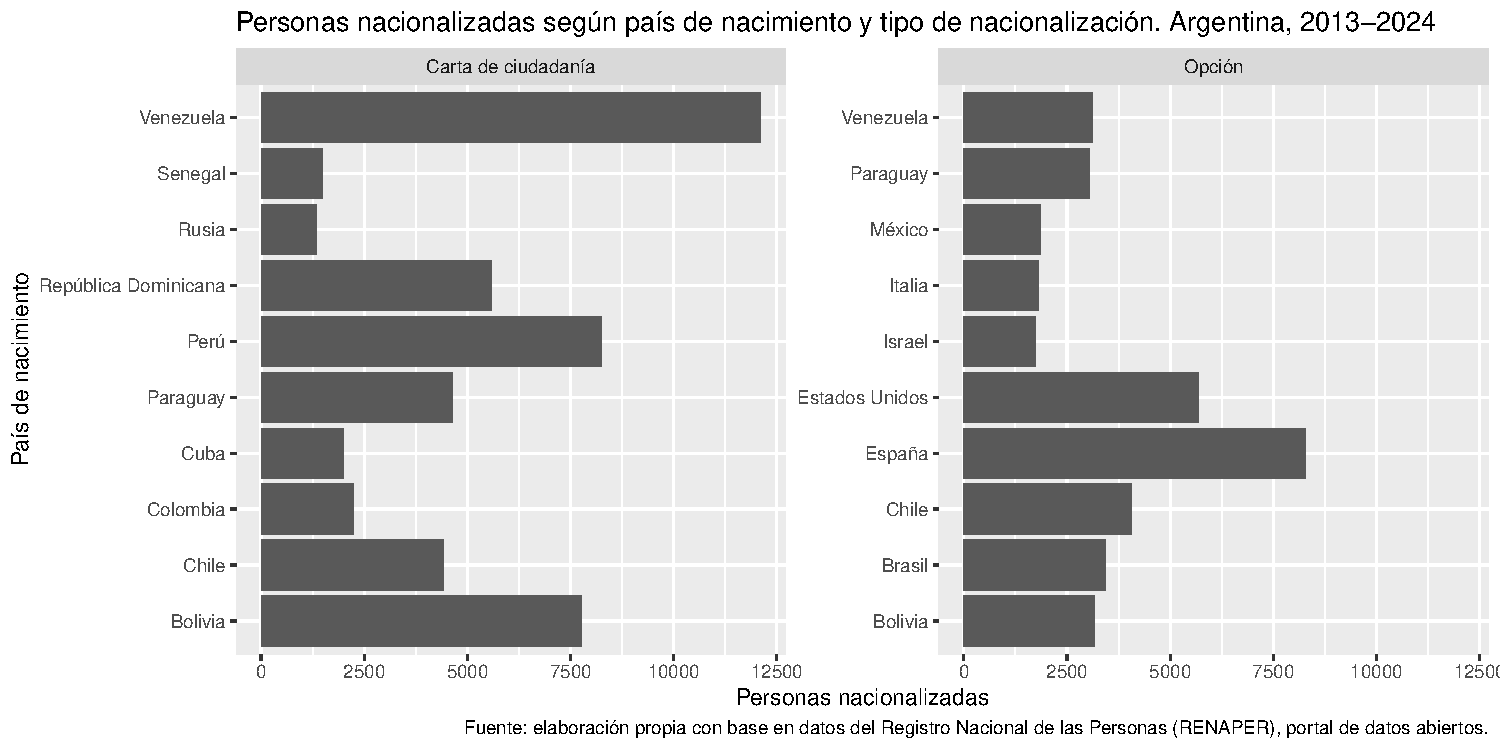
\includegraphics{tp1_files/figure-pdf/represent-barras-1.pdf}

\paragraph{\texorpdfstring{Evolución anual de los cinco principales
países
(\texttt{datos\_b})}{Evolución anual de los cinco principales países (datos\_b)}}\label{evoluciuxf3n-anual-de-los-cinco-principales-pauxedses-datos_b}

Para mostrar la evolución en el tiempo se elabora un gráfico de líneas
con puntos para cada vía de acceso a la nacionalidad: la línea muestra
la tendencia y los puntos señalan el valor de cada año, lo que facilita
identificar cambios puntuales. Se limita a los cinco principales países
de cada vía porque con más series el gráfico se vuelve difícil de leer.

A diferencia de las barras, donde los totales de ambas vías son
comparables, en la serie los volúmenes anuales difieren mucho (Venezuela
supera las 4.000 personas en carta de ciudadanía, mientras que en opción
ningún país alcanza las 1.400). Por eso cada vía tiene su propia escala,
y los valores se comparan dentro de cada vía y no entre ellas.

\begin{Shaded}
\begin{Highlighting}[]
\NormalTok{datos\_b }\SpecialCharTok{|\textgreater{}} 
  \FunctionTok{filter}\NormalTok{(tipo }\SpecialCharTok{==} \StringTok{"Carta de ciudadanía"}\NormalTok{) }\SpecialCharTok{|\textgreater{}} 
  \FunctionTok{ggplot}\NormalTok{(}\FunctionTok{aes}\NormalTok{(}\FunctionTok{as.factor}\NormalTok{(anio), }
\NormalTok{             cantidad, }
             \AttributeTok{group =}\NormalTok{ pais,}
             \AttributeTok{color =}\NormalTok{ pais)) }\SpecialCharTok{+}
  \FunctionTok{geom\_line}\NormalTok{(}\AttributeTok{linewidth =} \DecValTok{1}\NormalTok{) }\SpecialCharTok{+}
  \FunctionTok{geom\_point}\NormalTok{(}\AttributeTok{size =} \DecValTok{2}\NormalTok{) }\SpecialCharTok{+}
    \FunctionTok{labs}\NormalTok{(}
  \AttributeTok{title =} \StringTok{"Personas nacionalizadas por carta de ciudadanía según país de nacimiento"}\NormalTok{,}
  \AttributeTok{subtitle =} \StringTok{"Cinco principales países. Argentina, 2013–2024"}\NormalTok{,}
      \AttributeTok{y =} \StringTok{"Personas nacionalizadas"}\NormalTok{,}
      \AttributeTok{x =}  \StringTok{"Año de trámite primer DNI"}\NormalTok{,}
    \AttributeTok{color =} \StringTok{"País de nacimiento"}\NormalTok{,}
    \AttributeTok{caption =} \StringTok{"Fuente: elaboración propia con base en datos del Registro Nacional de las Personas (RENAPER), portal de datos abiertos."}
\NormalTok{  )}
\end{Highlighting}
\end{Shaded}

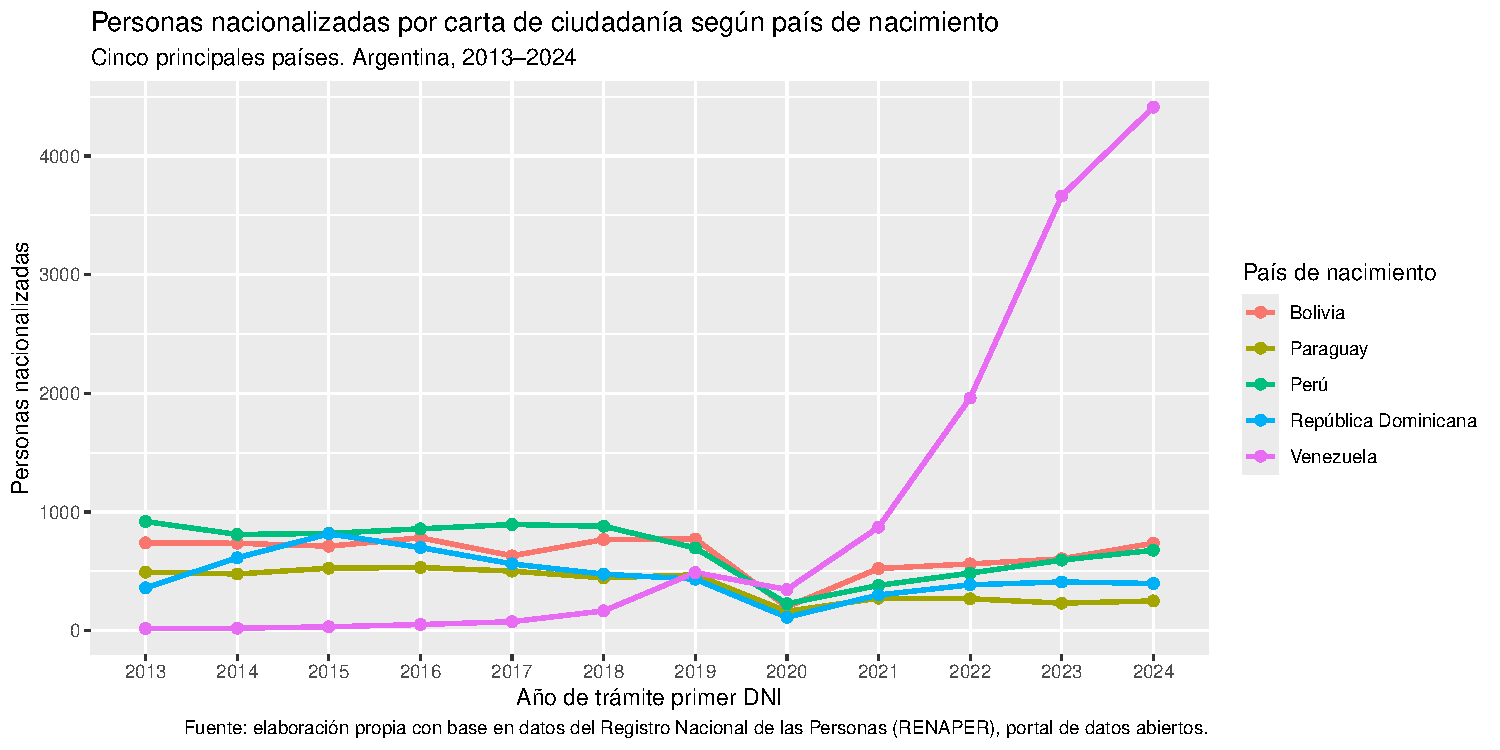
\includegraphics{tp1_files/figure-pdf/represent-serie1-1.pdf}

\begin{Shaded}
\begin{Highlighting}[]
\NormalTok{datos\_b }\SpecialCharTok{|\textgreater{}} 
  \FunctionTok{filter}\NormalTok{(tipo }\SpecialCharTok{==} \StringTok{"Opción"}\NormalTok{) }\SpecialCharTok{|\textgreater{}} 
  \FunctionTok{ggplot}\NormalTok{(}\FunctionTok{aes}\NormalTok{(}\FunctionTok{as.factor}\NormalTok{(anio), }
\NormalTok{             cantidad, }
             \AttributeTok{group =}\NormalTok{ pais,}
             \AttributeTok{color =}\NormalTok{ pais)) }\SpecialCharTok{+}
  \FunctionTok{geom\_line}\NormalTok{(}\AttributeTok{linewidth =} \DecValTok{1}\NormalTok{) }\SpecialCharTok{+}
  \FunctionTok{geom\_point}\NormalTok{(}\AttributeTok{size =} \DecValTok{2}\NormalTok{) }\SpecialCharTok{+}
  \FunctionTok{labs}\NormalTok{(}
    \AttributeTok{title =} \StringTok{"Personas nacionalizadas por opción según país de nacimiento"}\NormalTok{,}
    \AttributeTok{subtitle =} \StringTok{"Cinco principales países. Argentina, 2013–2024"}\NormalTok{,}
      \AttributeTok{y =} \StringTok{"Personas nacionalizadas"}\NormalTok{,}
      \AttributeTok{x =}  \StringTok{"Año de trámite primer DNI"}\NormalTok{,}
    \AttributeTok{color =} \StringTok{"País de nacimiento"}\NormalTok{,}
    \AttributeTok{caption =} \StringTok{"Fuente: elaboración propia con base en datos del Registro Nacional de las Personas (RENAPER), portal de datos abiertos."}
\NormalTok{  )}
\end{Highlighting}
\end{Shaded}

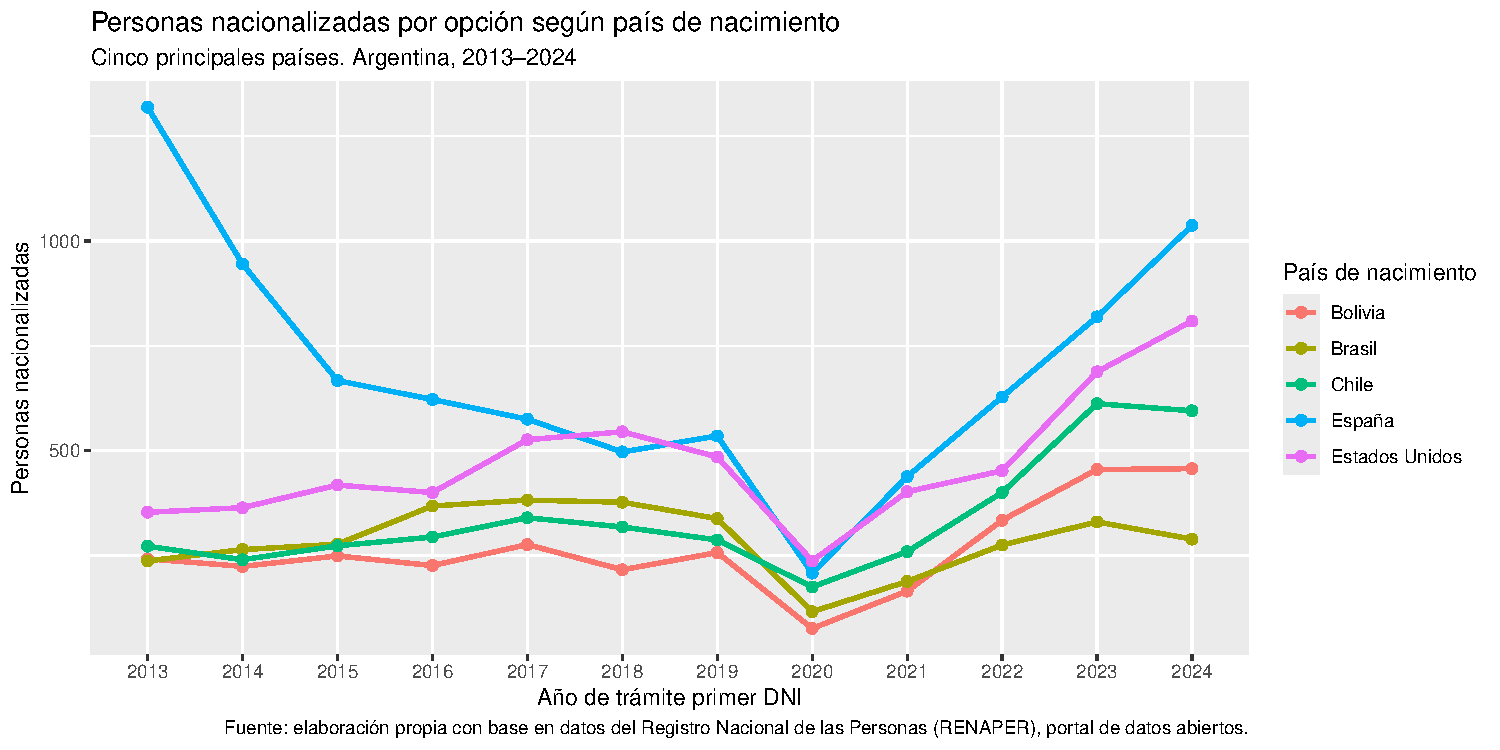
\includegraphics{tp1_files/figure-pdf/represent-serie2-1.pdf}

Estas versiones base permiten identificar los aspectos a mejorar en la
etapa siguiente: themes, paleta de colores, escalas de los ejes, entre
otros.

\subsubsection{\texorpdfstring{6. Refinar
(\emph{Refine})}{6. Refinar (Refine)}}\label{refinar-refine}

\paragraph{\texorpdfstring{Diez principales países por vía de acceso
(\texttt{datos\_a})}{Diez principales países por vía de acceso (datos\_a)}}\label{diez-principales-pauxedses-por-vuxeda-de-acceso-datos_a-1}

\begin{Shaded}
\begin{Highlighting}[]
\NormalTok{datos\_a }\SpecialCharTok{|\textgreater{}}
  \FunctionTok{mutate}\NormalTok{(}\AttributeTok{pais =} \FunctionTok{reorder\_within}\NormalTok{(pais, total, tipo)) }\SpecialCharTok{|\textgreater{}}
  \FunctionTok{ggplot}\NormalTok{(}\FunctionTok{aes}\NormalTok{(total, pais, }\AttributeTok{fill =}\NormalTok{ tipo)) }\SpecialCharTok{+}
  \FunctionTok{geom\_col}\NormalTok{() }\SpecialCharTok{+}
   \FunctionTok{geom\_text}\NormalTok{(}
    \FunctionTok{aes}\NormalTok{(}\AttributeTok{label =} \FunctionTok{number}\NormalTok{(total, }\AttributeTok{big.mark =} \StringTok{"."}\NormalTok{, }\AttributeTok{decimal.mark =} \StringTok{","}\NormalTok{), }\AttributeTok{color =}\NormalTok{ tipo),}
    \AttributeTok{hjust =} \FloatTok{1.1}\NormalTok{,}
    \AttributeTok{size =} \DecValTok{3}\NormalTok{) }\SpecialCharTok{+}
  \FunctionTok{scale\_y\_reordered}\NormalTok{() }\SpecialCharTok{+}
  \FunctionTok{scale\_fill\_manual}\NormalTok{(}\AttributeTok{values =} \FunctionTok{c}\NormalTok{(}\StringTok{"\#003049"}\NormalTok{, }\StringTok{"\#669BBC"}\NormalTok{), }\AttributeTok{guide =} \StringTok{"none"}\NormalTok{) }\SpecialCharTok{+}
  \FunctionTok{scale\_color\_manual}\NormalTok{(}\AttributeTok{values =} \FunctionTok{c}\NormalTok{(}\StringTok{"white"}\NormalTok{, }\StringTok{"black"}\NormalTok{), }\AttributeTok{guide =} \StringTok{"none"}\NormalTok{) }\SpecialCharTok{+}
  \FunctionTok{facet\_wrap}\NormalTok{(}\SpecialCharTok{\textasciitilde{}}\NormalTok{ tipo, }\AttributeTok{scales =} \StringTok{"free\_y"}\NormalTok{) }\SpecialCharTok{+}
  \FunctionTok{labs}\NormalTok{(}
    \AttributeTok{title =} \StringTok{"Personas nacionalizadas según país de nacimiento y tipo de nacionalización. Argentina, 2013–2024"}\NormalTok{,}
      \AttributeTok{x =} \StringTok{"Personas nacionalizadas"}\NormalTok{,}
      \AttributeTok{y =}  \StringTok{"País de nacimiento"}\NormalTok{,}
    \AttributeTok{caption =} \StringTok{"Fuente: elaboración propia con base en datos del Registro Nacional de las Personas (RENAPER), portal de datos abiertos."}
\NormalTok{  ) }\SpecialCharTok{+}
  \FunctionTok{theme\_bw}\NormalTok{()}
\end{Highlighting}
\end{Shaded}

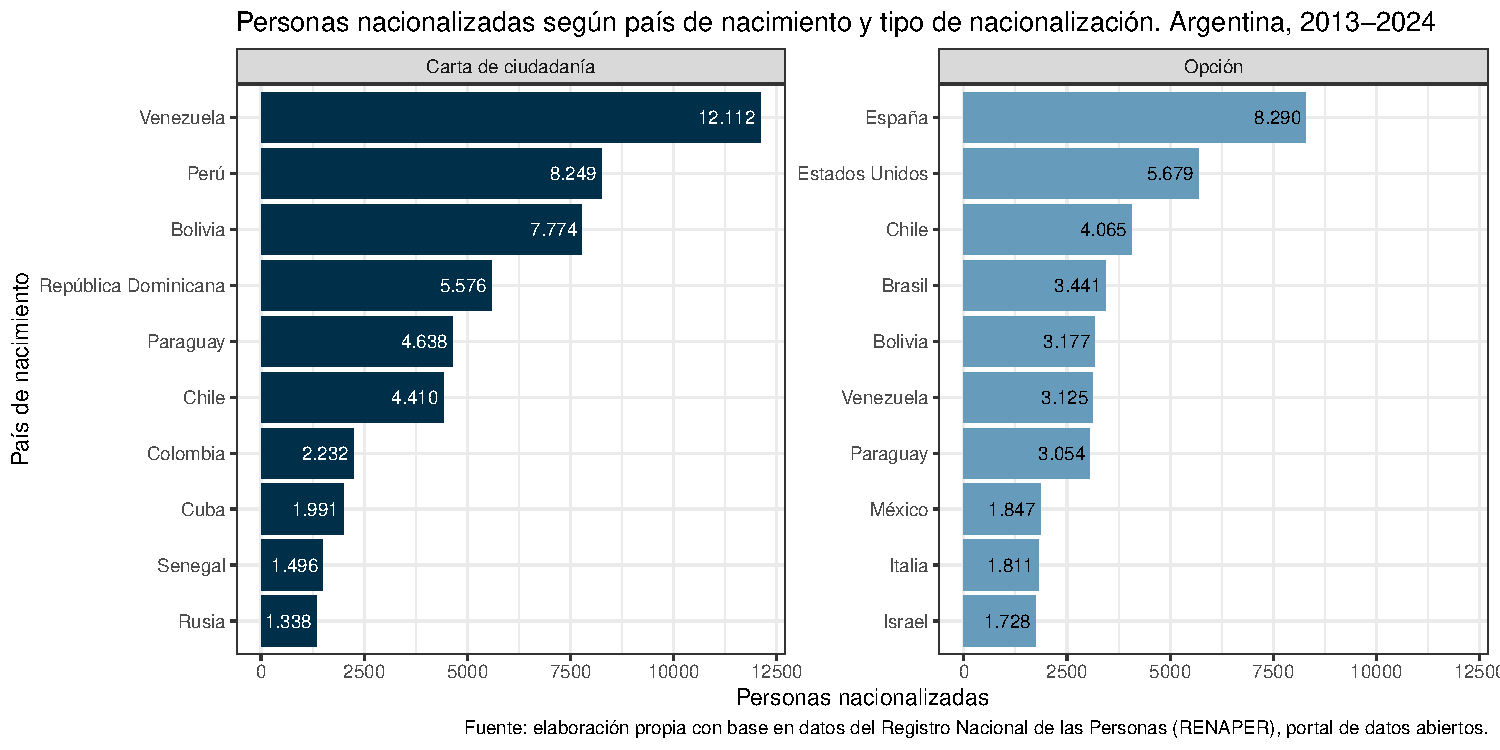
\includegraphics{tp1_files/figure-pdf/refine-barras-1.pdf}

\paragraph{\texorpdfstring{Evolución anual de los cinco principales
países
(\texttt{datos\_b})}{Evolución anual de los cinco principales países (datos\_b)}}\label{evoluciuxf3n-anual-de-los-cinco-principales-pauxedses-datos_b-1}

\begin{Shaded}
\begin{Highlighting}[]
\NormalTok{datos\_b }\SpecialCharTok{|\textgreater{}} 
  \FunctionTok{filter}\NormalTok{(tipo }\SpecialCharTok{==} \StringTok{"Carta de ciudadanía"}\NormalTok{) }\SpecialCharTok{|\textgreater{}} 
  \FunctionTok{ggplot}\NormalTok{(}\FunctionTok{aes}\NormalTok{(}\FunctionTok{as.factor}\NormalTok{(anio), }
\NormalTok{             cantidad, }
             \AttributeTok{group =}\NormalTok{ pais,}
             \AttributeTok{color =}\NormalTok{ pais)) }\SpecialCharTok{+}
  \FunctionTok{geom\_line}\NormalTok{(}\AttributeTok{linewidth =} \DecValTok{1}\NormalTok{) }\SpecialCharTok{+}
  \FunctionTok{geom\_point}\NormalTok{(}\AttributeTok{size =} \DecValTok{2}\NormalTok{) }\SpecialCharTok{+}
  \FunctionTok{scale\_y\_continuous}\NormalTok{(}\AttributeTok{limits =} \FunctionTok{c}\NormalTok{(}\DecValTok{0}\NormalTok{, }\DecValTok{5000}\NormalTok{)) }\SpecialCharTok{+} 
  \FunctionTok{scale\_color\_brewer}\NormalTok{(}\AttributeTok{palette =} \StringTok{"Set1"}\NormalTok{) }\SpecialCharTok{+}
    \FunctionTok{labs}\NormalTok{(}
  \AttributeTok{title =} \StringTok{"Personas nacionalizadas por carta de ciudadanía según país de nacimiento"}\NormalTok{,}
  \AttributeTok{subtitle =} \StringTok{"Cinco principales países. Argentina, 2013–2024"}\NormalTok{,}
      \AttributeTok{y =} \StringTok{"Personas nacionalizadas"}\NormalTok{,}
      \AttributeTok{x =}  \StringTok{"Año de trámite primer DNI"}\NormalTok{,}
    \AttributeTok{color =} \StringTok{"País de nacimiento"}\NormalTok{,}
    \AttributeTok{caption =} \StringTok{"Fuente: elaboración propia con base en datos del Registro Nacional de las Personas (RENAPER), portal de datos abiertos."}
\NormalTok{  ) }\SpecialCharTok{+}
  \FunctionTok{theme\_bw}\NormalTok{() }\SpecialCharTok{+}
    \FunctionTok{theme}\NormalTok{(}
    \AttributeTok{legend.position =} \StringTok{"bottom"}
\NormalTok{  )}
\end{Highlighting}
\end{Shaded}

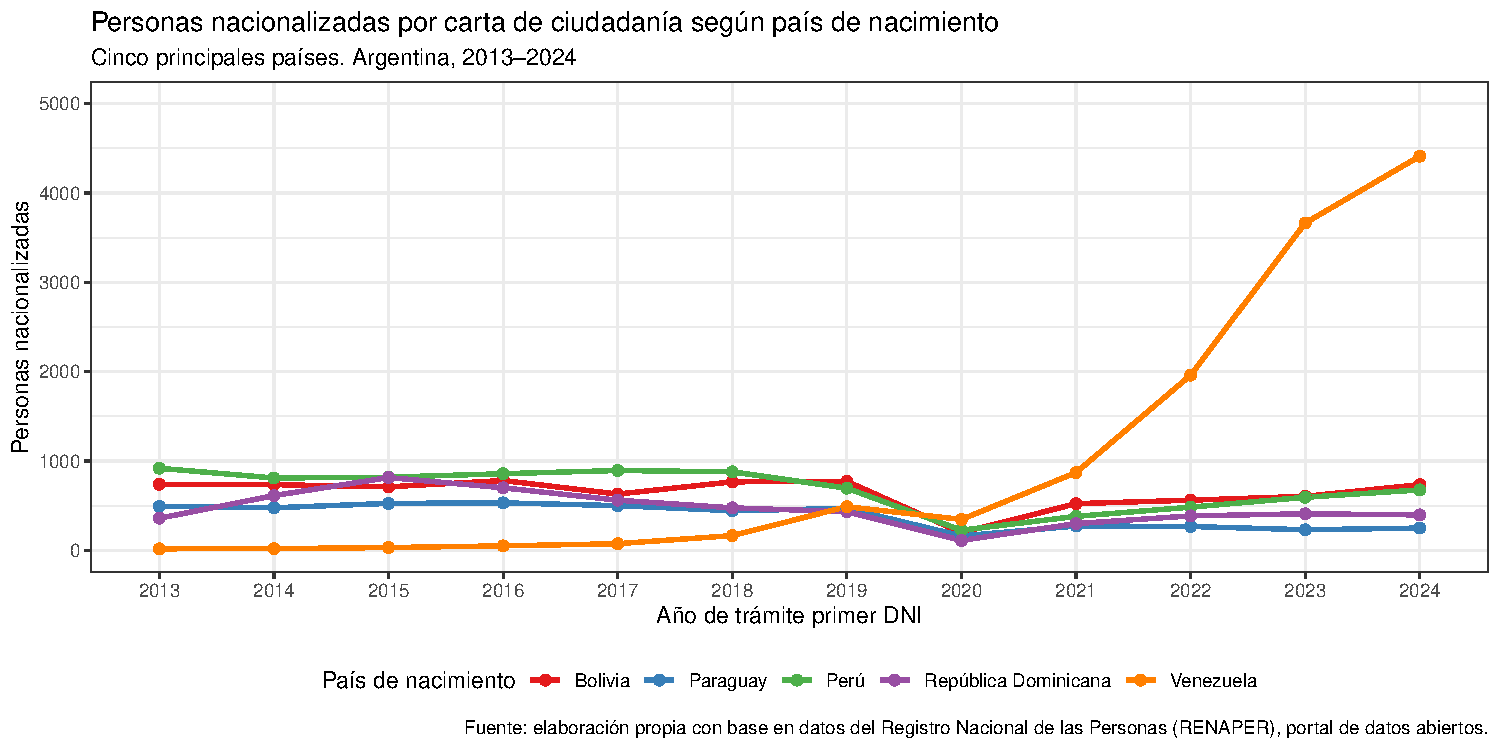
\includegraphics{tp1_files/figure-pdf/serie-ciudadania-1.pdf}

\begin{Shaded}
\begin{Highlighting}[]
\NormalTok{datos\_b }\SpecialCharTok{|\textgreater{}} 
  \FunctionTok{filter}\NormalTok{(tipo }\SpecialCharTok{==} \StringTok{"Opción"}\NormalTok{) }\SpecialCharTok{|\textgreater{}} 
  \FunctionTok{ggplot}\NormalTok{(}\FunctionTok{aes}\NormalTok{(}\FunctionTok{as.factor}\NormalTok{(anio), }
\NormalTok{             cantidad, }
             \AttributeTok{group =}\NormalTok{ pais,}
             \AttributeTok{color =}\NormalTok{ pais)) }\SpecialCharTok{+}
  \FunctionTok{geom\_line}\NormalTok{(}\AttributeTok{linewidth =} \DecValTok{1}\NormalTok{) }\SpecialCharTok{+}
  \FunctionTok{geom\_point}\NormalTok{(}\AttributeTok{size =} \DecValTok{2}\NormalTok{) }\SpecialCharTok{+}
  \FunctionTok{scale\_y\_continuous}\NormalTok{(}\AttributeTok{limits =} \FunctionTok{c}\NormalTok{(}\DecValTok{0}\NormalTok{, }\DecValTok{1500}\NormalTok{)) }\SpecialCharTok{+} 
  \FunctionTok{scale\_color\_brewer}\NormalTok{(}\AttributeTok{palette =} \StringTok{"Dark2"}\NormalTok{) }\SpecialCharTok{+}
  \FunctionTok{labs}\NormalTok{(}
    \AttributeTok{title =} \StringTok{"Personas nacionalizadas por opción según país de nacimiento"}\NormalTok{,}
    \AttributeTok{subtitle =} \StringTok{"Cinco principales países. Argentina, 2013–2024"}\NormalTok{,}
      \AttributeTok{y =} \StringTok{"Personas nacionalizadas"}\NormalTok{,}
      \AttributeTok{x =}  \StringTok{"Año de trámite primer DNI"}\NormalTok{,}
    \AttributeTok{color =} \StringTok{"País de nacimiento"}\NormalTok{,}
    \AttributeTok{caption =} \StringTok{"Fuente: elaboración propia con base en datos del Registro Nacional de las Personas (RENAPER), portal de datos abiertos."}\NormalTok{) }\SpecialCharTok{+}
  \FunctionTok{theme\_bw}\NormalTok{() }\SpecialCharTok{+}
    \FunctionTok{theme}\NormalTok{(}
    \AttributeTok{legend.position =} \StringTok{"bottom"}
\NormalTok{  )}
\end{Highlighting}
\end{Shaded}

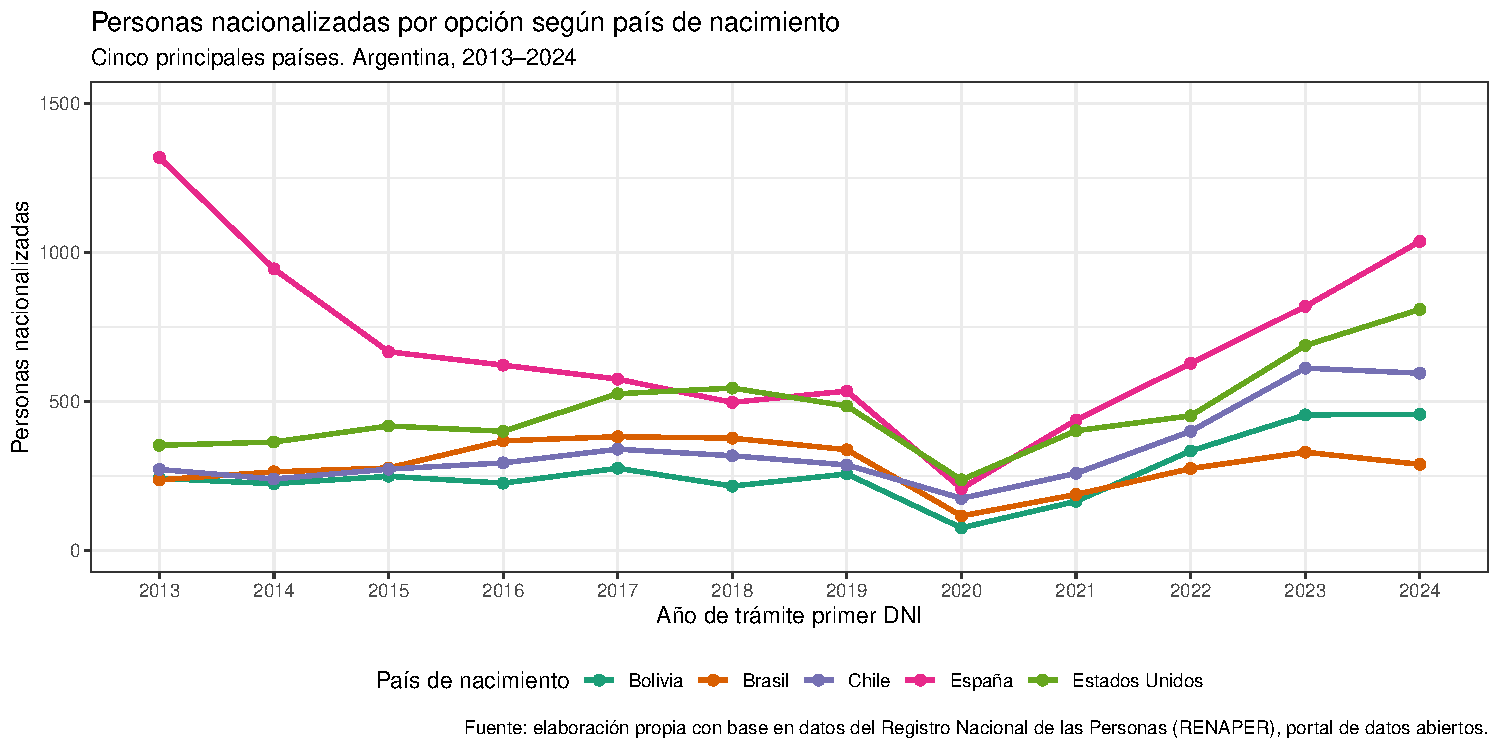
\includegraphics{tp1_files/figure-pdf/serie-opcion-1.pdf}

\subsection{Conclusiones}\label{conclusiones}

El análisis visual permite responder la pregunta planteada: entre 2013 y
2024, las personas que se nacionalizaron en Argentina provienen de
orígenes distintos según la vía de acceso a la nacionalidad, y la
composición de esos orígenes cambió de forma marcada a partir de la
pandemia de COVID-19.

En el período analizado, 108.918 personas realizaron su primer DNI como
argentinas. Ambas vías tienen un peso similar en ese total, pero sus
perfiles de origen difieren: solo Bolivia, Chile, Paraguay y Venezuela
figuran entre los diez principales países de las dos vías. La carta de
ciudadanía se concentra en países latinoamericanos y del Caribe, con
Venezuela, Perú y Bolivia a la cabeza, mientras que la opción,
encabezada por España y Estados Unidos, presenta una distribución más
diversificada, con países como México, Italia e Israel.

En cuanto a la evolución temporal, ambas vías se mantienen estables
entre 2013 y 2019, caen abruptamente en 2020, probablemente por la
interrupción de trámites presenciales durante la pandemia, y se
recuperan con fuerza a partir de 2021. Ese crecimiento reciente se
explica principalmente por Venezuela en la carta de ciudadanía, que pasa
de 19 personas en 2013 a 4.411 en 2024, mientras disminuyen orígenes
tradicionales como Perú y Paraguay. En la opción crecen Estados Unidos y
Chile, y España, aunque se mantiene como principal origen, desciende.

Estas diferencias son consistentes con la naturaleza de cada vía: la
carta de ciudadanía refleja trayectorias de inmigración y residencia en
el país, mientras que la opción expresa en mayor medida vínculos de
filiación con la población argentina, incluida la emigrada. Sin embargo,
la presencia de países limítrofes en ambas vías muestra que la
distinción no es tajante y que la movilidad regional también se expresa
a través de la opción. Al mismo tiempo, los cambios observados recuerdan
que los fenómenos migratorios son dinámicos y responden a contextos
internacionales demográficos, sociales, económicos y políticos, como lo
muestran el crecimiento de la población venezolana, la presencia de
orígenes como Senegal o Rusia y los destinos de la emigración argentina
que se reflejan en la opción. Comprender la evolución de las
nacionalizaciones requiere, por lo tanto, situarla en esos contextos.

\subsection{Referencias}\label{referencias}

\subsubsection{Bibliografía}\label{bibliografuxeda}

Fry, B. (2008). \emph{Visualizing Data: Exploring and Explaining Data
with the Processing Environment}. O'Reilly Media.

\subsubsection{Normativa}\label{normativa}

Ley N° 346 de Ciudadanía y Naturalización. (1869). República Argentina.

Decreto N° 3213/1984. Reglamentación de la Ley N° 346. República
Argentina.

Decreto N° 1501/2009. República Argentina.

Registro Nacional de las Personas. Resolución N° 1800/2009.

Registro Nacional de las Personas. Resolución N° 585/2012.

\subsubsection{Fuentes de datos}\label{fuentes-de-datos}

Registro Nacional de las Personas (RENAPER). (s. f.). \emph{Cantidad de
trámites de DNI argentino por nacionalidad, país y año} {[}Conjunto de
datos{]}. Portal de datos abiertos del RENAPER. Recuperado el 20 de
octubre de 2026, de
https://datosabiertos.renaper.gob.ar/Cantidad\_de\_tramites\_de\_DNI\_argentino\_por\_nacionalidad\_pais\_anio.csv

Registro Nacional de las Personas (RENAPER). (s. f.). \emph{Estadística
de población}.
https://www.argentina.gob.ar/interior/renaper/estadistica-de-poblacion

\subsubsection{Software}\label{software}

R Core Team. (2025). \emph{R: A Language and Environment for Statistical
Computing}. R Foundation for Statistical Computing.
https://www.R-project.org/




\end{document}
